\documentclass[twoside]{book}

% Packages required by doxygen
\usepackage{fixltx2e}
\usepackage{calc}
\usepackage{doxygen}
\usepackage[export]{adjustbox} % also loads graphicx
\usepackage{graphicx}
\usepackage[utf8]{inputenc}
\usepackage{makeidx}
\usepackage{multicol}
\usepackage{multirow}
\PassOptionsToPackage{warn}{textcomp}
\usepackage{textcomp}
\usepackage[nointegrals]{wasysym}
\usepackage[table]{xcolor}

% Font selection
\usepackage[T1]{fontenc}
\usepackage[scaled=.90]{helvet}
\usepackage{courier}
\usepackage{amssymb}
\usepackage{sectsty}
\renewcommand{\familydefault}{\sfdefault}
\allsectionsfont{%
  \fontseries{bc}\selectfont%
  \color{darkgray}%
}
\renewcommand{\DoxyLabelFont}{%
  \fontseries{bc}\selectfont%
  \color{darkgray}%
}
\newcommand{\+}{\discretionary{\mbox{\scriptsize$\hookleftarrow$}}{}{}}

% Page & text layout
\usepackage{geometry}
\geometry{%
  a4paper,%
  top=2.5cm,%
  bottom=2.5cm,%
  left=2.5cm,%
  right=2.5cm%
}
\tolerance=750
\hfuzz=15pt
\hbadness=750
\setlength{\emergencystretch}{15pt}
\setlength{\parindent}{0cm}
\setlength{\parskip}{0.2cm}
\makeatletter
\renewcommand{\paragraph}{%
  \@startsection{paragraph}{4}{0ex}{-1.0ex}{1.0ex}{%
    \normalfont\normalsize\bfseries\SS@parafont%
  }%
}
\renewcommand{\subparagraph}{%
  \@startsection{subparagraph}{5}{0ex}{-1.0ex}{1.0ex}{%
    \normalfont\normalsize\bfseries\SS@subparafont%
  }%
}
\makeatother

% Headers & footers
\usepackage{fancyhdr}
\pagestyle{fancyplain}
\fancyhead[LE]{\fancyplain{}{\bfseries\thepage}}
\fancyhead[CE]{\fancyplain{}{}}
\fancyhead[RE]{\fancyplain{}{\bfseries\leftmark}}
\fancyhead[LO]{\fancyplain{}{\bfseries\rightmark}}
\fancyhead[CO]{\fancyplain{}{}}
\fancyhead[RO]{\fancyplain{}{\bfseries\thepage}}
\fancyfoot[LE]{\fancyplain{}{}}
\fancyfoot[CE]{\fancyplain{}{}}
\fancyfoot[RE]{\fancyplain{}{\bfseries\scriptsize Generated on Wed Nov 18 2015 13\+:37\+:08 for pylink\+Crawler by Doxygen }}
\fancyfoot[LO]{\fancyplain{}{\bfseries\scriptsize Generated on Wed Nov 18 2015 13\+:37\+:08 for pylink\+Crawler by Doxygen }}
\fancyfoot[CO]{\fancyplain{}{}}
\fancyfoot[RO]{\fancyplain{}{}}
\renewcommand{\footrulewidth}{0.4pt}
\renewcommand{\chaptermark}[1]{%
  \markboth{#1}{}%
}
\renewcommand{\sectionmark}[1]{%
  \markright{\thesection\ #1}%
}

% Indices & bibliography
\usepackage{natbib}
\usepackage[titles]{tocloft}
\setcounter{tocdepth}{3}
\setcounter{secnumdepth}{5}
\makeindex

% Hyperlinks (required, but should be loaded last)
\usepackage{ifpdf}
\ifpdf
  \usepackage[pdftex,pagebackref=true]{hyperref}
\else
  \usepackage[ps2pdf,pagebackref=true]{hyperref}
\fi
\hypersetup{%
  colorlinks=true,%
  linkcolor=blue,%
  citecolor=blue,%
  unicode%
}

% Custom commands
\newcommand{\clearemptydoublepage}{%
  \newpage{\pagestyle{empty}\cleardoublepage}%
}

\usepackage{caption}
\captionsetup{labelsep=space,justification=centering,font={bf},singlelinecheck=off,skip=4pt,position=top}

%===== C O N T E N T S =====

\begin{document}

% Titlepage & ToC
\hypersetup{pageanchor=false,
             bookmarks=true,
             bookmarksnumbered=true,
             pdfencoding=unicode
            }
\pagenumbering{roman}
\begin{titlepage}
\vspace*{7cm}
\begin{center}%
{\Large pylink\+Crawler }\\
\vspace*{1cm}
{\large Generated by Doxygen 1.8.11}\\
\vspace*{0.5cm}
{\small Wed Nov 18 2015 13:37:08}\\
\end{center}
\end{titlepage}
\clearemptydoublepage
\tableofcontents
\clearemptydoublepage
\pagenumbering{arabic}
\hypersetup{pageanchor=true}

%--- Begin generated contents ---
\chapter{Hierarchical Index}
\section{Class Hierarchy}
This inheritance list is sorted roughly, but not completely, alphabetically\+:\begin{DoxyCompactList}
\item object\begin{DoxyCompactList}
\item \contentsline{section}{pylinkvalidator.\+P\+OC Code.\+Web\+\_\+\+Crawler.\+H\+T\+M\+L\+\_\+corrector\+\_\+help}{\pageref{classpylinkvalidator_1_1_p_o_c_01_code_1_1_web___crawler_1_1_h_t_m_l__corrector__help}}{}
\item \contentsline{section}{pylinkvalidator.\+P\+OC Code.\+Web\+\_\+\+Crawler.\+Web\+\_\+\+Crawler}{\pageref{classpylinkvalidator_1_1_p_o_c_01_code_1_1_web___crawler_1_1_web___crawler}}{}
\item \contentsline{section}{pylinkvalidator.\+P\+OC Code.\+Web\+\_\+\+Crawler\+\_\+\+P\+O\+C.\+Web\+\_\+\+Crawler\+\_\+\+P\+OC}{\pageref{classpylinkvalidator_1_1_p_o_c_01_code_1_1_web___crawler___p_o_c_1_1_web___crawler___p_o_c}}{}
\item \contentsline{section}{pylinkvalidator.\+Web\+Handy\+Tool.\+download.\+download}{\pageref{classpylinkvalidator_1_1_web_handy_tool_1_1download_1_1download}}{}
\item \contentsline{section}{pylinkvalidator.\+Web\+Handy\+Tool.\+errors.\+errors}{\pageref{classpylinkvalidator_1_1_web_handy_tool_1_1errors_1_1errors}}{}
\item \contentsline{section}{pylinkvalidator.\+Web\+Handy\+Tool.\+link\+Search\+Algos.\+link\+Search\+Algos}{\pageref{classpylinkvalidator_1_1_web_handy_tool_1_1link_search_algos_1_1link_search_algos}}{}
\item \contentsline{section}{pylinkvalidator.\+Web\+Handy\+Tool.\+parsers.\+parsers}{\pageref{classpylinkvalidator_1_1_web_handy_tool_1_1parsers_1_1parsers}}{}
\item \contentsline{section}{pylinkvalidator.\+Web\+Handy\+Tool.\+search.\+search}{\pageref{classpylinkvalidator_1_1_web_handy_tool_1_1search_1_1search}}{}
\item \contentsline{section}{pylinkvalidator.\+Web\+Handy\+Tool.\+url\+Corrector.\+H\+T\+M\+L\+\_\+corrector\+\_\+help}{\pageref{classpylinkvalidator_1_1_web_handy_tool_1_1url_corrector_1_1_h_t_m_l__corrector__help}}{}
\item \contentsline{section}{pylinkvalidator.\+Web\+Handy\+Tool.\+url\+Corrector.\+url\+Corrector}{\pageref{classpylinkvalidator_1_1_web_handy_tool_1_1url_corrector_1_1url_corrector}}{}
\item \contentsline{section}{pylinkvalidator.\+Web\+Handy\+Tool.\+Web\+\_\+\+Crawler.\+Web\+\_\+\+Crawler}{\pageref{classpylinkvalidator_1_1_web_handy_tool_1_1_web___crawler_1_1_web___crawler}}{}
\end{DoxyCompactList}
\item T\+C\+P\+Server\begin{DoxyCompactList}
\item \contentsline{section}{pylinkvalidator.\+Web\+Handy\+Tool.\+tests.\+Threaded\+T\+C\+P\+Server}{\pageref{classpylinkvalidator_1_1_web_handy_tool_1_1tests_1_1_threaded_t_c_p_server}}{}
\end{DoxyCompactList}
\item Test\+Case\begin{DoxyCompactList}
\item \contentsline{section}{pylinkvalidator.\+Web\+Handy\+Tool.\+tests.\+crawler\+Test}{\pageref{classpylinkvalidator_1_1_web_handy_tool_1_1tests_1_1crawler_test}}{}
\item \contentsline{section}{pylinkvalidator.\+Web\+Handy\+Tool.\+tests.\+search\+Test}{\pageref{classpylinkvalidator_1_1_web_handy_tool_1_1tests_1_1search_test}}{}
\item \contentsline{section}{pylinkvalidator.\+Web\+Handy\+Tool.\+tests.\+url\+Corrector\+Test}{\pageref{classpylinkvalidator_1_1_web_handy_tool_1_1tests_1_1url_corrector_test}}{}
\item \contentsline{section}{Test\+String.\+Test\+String\+Methods}{\pageref{class_test_string_1_1_test_string_methods}}{}
\end{DoxyCompactList}
\item Threading\+Mix\+In\begin{DoxyCompactList}
\item \contentsline{section}{pylinkvalidator.\+Web\+Handy\+Tool.\+tests.\+Threaded\+T\+C\+P\+Server}{\pageref{classpylinkvalidator_1_1_web_handy_tool_1_1tests_1_1_threaded_t_c_p_server}}{}
\end{DoxyCompactList}
\end{DoxyCompactList}

\chapter{Class Index}
\section{Class List}
Here are the classes, structs, unions and interfaces with brief descriptions\+:\begin{DoxyCompactList}
\item\contentsline{section}{\hyperlink{class_web___crawler_1_1_h_t_m_l__corrector__help}{Web\+\_\+\+Crawler.\+H\+T\+M\+L\+\_\+corrector\+\_\+help} }{\pageref{class_web___crawler_1_1_h_t_m_l__corrector__help}}{}
\item\contentsline{section}{\hyperlink{class_test_string_1_1_test_string_methods}{Test\+String.\+Test\+String\+Methods} }{\pageref{class_test_string_1_1_test_string_methods}}{}
\item\contentsline{section}{\hyperlink{class_web___crawler_1_1_web___crawler}{Web\+\_\+\+Crawler.\+Web\+\_\+\+Crawler} }{\pageref{class_web___crawler_1_1_web___crawler}}{}
\item\contentsline{section}{\hyperlink{class_web___crawler___p_o_c_1_1_web___crawler___p_o_c}{Web\+\_\+\+Crawler\+\_\+\+P\+O\+C.\+Web\+\_\+\+Crawler\+\_\+\+P\+OC} }{\pageref{class_web___crawler___p_o_c_1_1_web___crawler___p_o_c}}{}
\end{DoxyCompactList}

\chapter{Class Documentation}
\hypertarget{class_web___crawler_1_1_h_t_m_l__corrector__help}{}\section{Web\+\_\+\+Crawler.\+H\+T\+M\+L\+\_\+corrector\+\_\+help Class Reference}
\label{class_web___crawler_1_1_h_t_m_l__corrector__help}\index{Web\+\_\+\+Crawler.\+H\+T\+M\+L\+\_\+corrector\+\_\+help@{Web\+\_\+\+Crawler.\+H\+T\+M\+L\+\_\+corrector\+\_\+help}}


Inheritance diagram for Web\+\_\+\+Crawler.\+H\+T\+M\+L\+\_\+corrector\+\_\+help\+:
\nopagebreak
\begin{figure}[H]
\begin{center}
\leavevmode
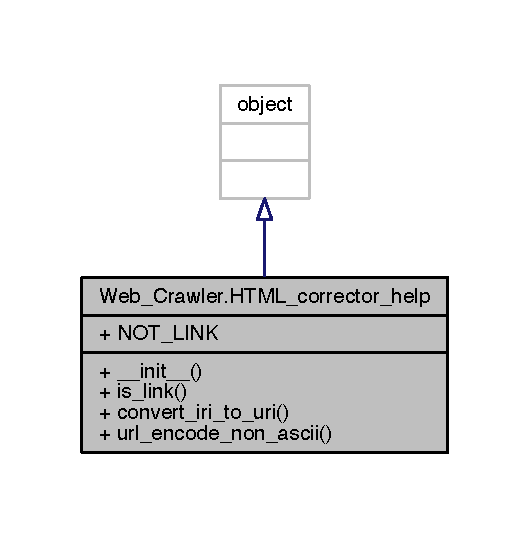
\includegraphics[width=254pt]{class_web___crawler_1_1_h_t_m_l__corrector__help__inherit__graph}
\end{center}
\end{figure}


Collaboration diagram for Web\+\_\+\+Crawler.\+H\+T\+M\+L\+\_\+corrector\+\_\+help\+:
\nopagebreak
\begin{figure}[H]
\begin{center}
\leavevmode
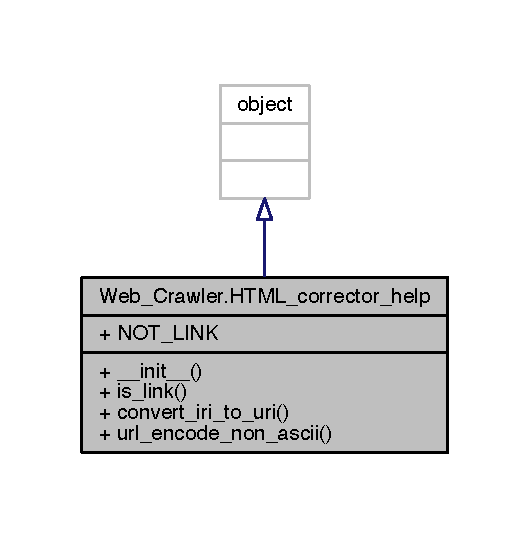
\includegraphics[width=254pt]{class_web___crawler_1_1_h_t_m_l__corrector__help__coll__graph}
\end{center}
\end{figure}
\subsection*{Public Member Functions}
\begin{DoxyCompactItemize}
\item 
def {\bfseries \+\_\+\+\_\+init\+\_\+\+\_\+} (self)\hypertarget{class_web___crawler_1_1_h_t_m_l__corrector__help_abd44f92aa00e86d2ba9a8867e646e3f7}{}\label{class_web___crawler_1_1_h_t_m_l__corrector__help_abd44f92aa00e86d2ba9a8867e646e3f7}

\item 
def \hyperlink{class_web___crawler_1_1_h_t_m_l__corrector__help_a28cd0ccee8404768e765043ada81176f}{is\+\_\+link} (self, url)
\item 
def \hyperlink{class_web___crawler_1_1_h_t_m_l__corrector__help_a71530aacd9f02ba14c0eb6683698dba9}{convert\+\_\+iri\+\_\+to\+\_\+uri} (self, url\+\_\+split)
\item 
def \hyperlink{class_web___crawler_1_1_h_t_m_l__corrector__help_ad8557b751c09dff4270255c85cfb9b36}{url\+\_\+encode\+\_\+non\+\_\+ascii} (self, url\+\_\+part)
\end{DoxyCompactItemize}
\subsection*{Public Attributes}
\begin{DoxyCompactItemize}
\item 
{\bfseries N\+O\+T\+\_\+\+L\+I\+NK}\hypertarget{class_web___crawler_1_1_h_t_m_l__corrector__help_a18b1945854173c1816b2d1eb0eef7528}{}\label{class_web___crawler_1_1_h_t_m_l__corrector__help_a18b1945854173c1816b2d1eb0eef7528}

\end{DoxyCompactItemize}


\subsection{Detailed Description}
\begin{DoxyVerb}Library of helper functions that are used by HTML corrector to
fix url links.
\end{DoxyVerb}
 

\subsection{Member Function Documentation}
\index{Web\+\_\+\+Crawler\+::\+H\+T\+M\+L\+\_\+corrector\+\_\+help@{Web\+\_\+\+Crawler\+::\+H\+T\+M\+L\+\_\+corrector\+\_\+help}!convert\+\_\+iri\+\_\+to\+\_\+uri@{convert\+\_\+iri\+\_\+to\+\_\+uri}}
\index{convert\+\_\+iri\+\_\+to\+\_\+uri@{convert\+\_\+iri\+\_\+to\+\_\+uri}!Web\+\_\+\+Crawler\+::\+H\+T\+M\+L\+\_\+corrector\+\_\+help@{Web\+\_\+\+Crawler\+::\+H\+T\+M\+L\+\_\+corrector\+\_\+help}}
\subsubsection[{convert\+\_\+iri\+\_\+to\+\_\+uri(self, url\+\_\+split)}]{\setlength{\rightskip}{0pt plus 5cm}def Web\+\_\+\+Crawler.\+H\+T\+M\+L\+\_\+corrector\+\_\+help.\+convert\+\_\+iri\+\_\+to\+\_\+uri (
\begin{DoxyParamCaption}
\item[{}]{self, }
\item[{}]{url\+\_\+split}
\end{DoxyParamCaption}
)}\hypertarget{class_web___crawler_1_1_h_t_m_l__corrector__help_a71530aacd9f02ba14c0eb6683698dba9}{}\label{class_web___crawler_1_1_h_t_m_l__corrector__help_a71530aacd9f02ba14c0eb6683698dba9}
\begin{DoxyVerb}Attempts to convert potential IRI to URI.

IRI may contain non-ascii characters.
:param url_split:
:return:
\end{DoxyVerb}
 

Here is the call graph for this function\+:
\nopagebreak
\begin{figure}[H]
\begin{center}
\leavevmode
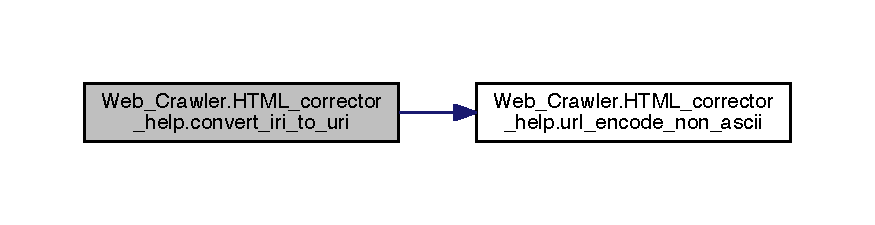
\includegraphics[width=350pt]{class_web___crawler_1_1_h_t_m_l__corrector__help_a71530aacd9f02ba14c0eb6683698dba9_cgraph}
\end{center}
\end{figure}


\index{Web\+\_\+\+Crawler\+::\+H\+T\+M\+L\+\_\+corrector\+\_\+help@{Web\+\_\+\+Crawler\+::\+H\+T\+M\+L\+\_\+corrector\+\_\+help}!is\+\_\+link@{is\+\_\+link}}
\index{is\+\_\+link@{is\+\_\+link}!Web\+\_\+\+Crawler\+::\+H\+T\+M\+L\+\_\+corrector\+\_\+help@{Web\+\_\+\+Crawler\+::\+H\+T\+M\+L\+\_\+corrector\+\_\+help}}
\subsubsection[{is\+\_\+link(self, url)}]{\setlength{\rightskip}{0pt plus 5cm}def Web\+\_\+\+Crawler.\+H\+T\+M\+L\+\_\+corrector\+\_\+help.\+is\+\_\+link (
\begin{DoxyParamCaption}
\item[{}]{self, }
\item[{}]{url}
\end{DoxyParamCaption}
)}\hypertarget{class_web___crawler_1_1_h_t_m_l__corrector__help_a28cd0ccee8404768e765043ada81176f}{}\label{class_web___crawler_1_1_h_t_m_l__corrector__help_a28cd0ccee8404768e765043ada81176f}
\begin{DoxyVerb}Return True if the url is not base 64 data or a local ref (#)

:param url:
:return Boolean either True or False:
\end{DoxyVerb}
 \index{Web\+\_\+\+Crawler\+::\+H\+T\+M\+L\+\_\+corrector\+\_\+help@{Web\+\_\+\+Crawler\+::\+H\+T\+M\+L\+\_\+corrector\+\_\+help}!url\+\_\+encode\+\_\+non\+\_\+ascii@{url\+\_\+encode\+\_\+non\+\_\+ascii}}
\index{url\+\_\+encode\+\_\+non\+\_\+ascii@{url\+\_\+encode\+\_\+non\+\_\+ascii}!Web\+\_\+\+Crawler\+::\+H\+T\+M\+L\+\_\+corrector\+\_\+help@{Web\+\_\+\+Crawler\+::\+H\+T\+M\+L\+\_\+corrector\+\_\+help}}
\subsubsection[{url\+\_\+encode\+\_\+non\+\_\+ascii(self, url\+\_\+part)}]{\setlength{\rightskip}{0pt plus 5cm}def Web\+\_\+\+Crawler.\+H\+T\+M\+L\+\_\+corrector\+\_\+help.\+url\+\_\+encode\+\_\+non\+\_\+ascii (
\begin{DoxyParamCaption}
\item[{}]{self, }
\item[{}]{url\+\_\+part}
\end{DoxyParamCaption}
)}\hypertarget{class_web___crawler_1_1_h_t_m_l__corrector__help_ad8557b751c09dff4270255c85cfb9b36}{}\label{class_web___crawler_1_1_h_t_m_l__corrector__help_ad8557b751c09dff4270255c85cfb9b36}
\begin{DoxyVerb}For each byte in url_part, if the byte is outside ascii range, quote the
byte. UTF characters that take two bytes will be correctly converted using
this technique.

We do not quote the whole url part because it might contain already quoted
characters, which would then be double-quoted.

The url part is converted from utf-8 and then to utf-8, which might not
always work if there is mixed or bad encoding.
:param url_part:
:return:
\end{DoxyVerb}
 

Here is the caller graph for this function\+:
\nopagebreak
\begin{figure}[H]
\begin{center}
\leavevmode
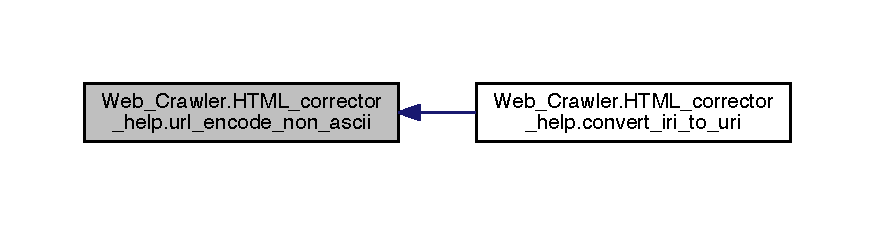
\includegraphics[width=350pt]{class_web___crawler_1_1_h_t_m_l__corrector__help_ad8557b751c09dff4270255c85cfb9b36_icgraph}
\end{center}
\end{figure}




The documentation for this class was generated from the following file\+:\begin{DoxyCompactItemize}
\item 
P\+O\+C Code/Web\+\_\+\+Crawler.\+py\end{DoxyCompactItemize}

\hypertarget{class_test_string_1_1_test_string_methods}{}\section{Test\+String.\+Test\+String\+Methods Class Reference}
\label{class_test_string_1_1_test_string_methods}\index{Test\+String.\+Test\+String\+Methods@{Test\+String.\+Test\+String\+Methods}}


Inheritance diagram for Test\+String.\+Test\+String\+Methods\+:
\nopagebreak
\begin{figure}[H]
\begin{center}
\leavevmode
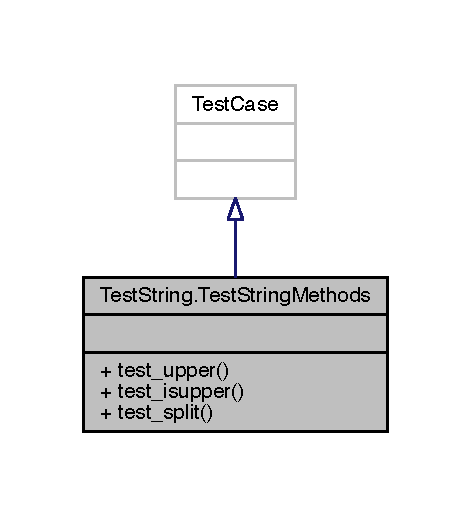
\includegraphics[width=226pt]{class_test_string_1_1_test_string_methods__inherit__graph}
\end{center}
\end{figure}


Collaboration diagram for Test\+String.\+Test\+String\+Methods\+:
\nopagebreak
\begin{figure}[H]
\begin{center}
\leavevmode
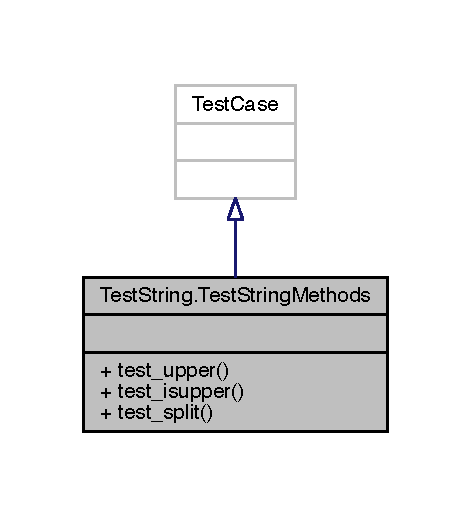
\includegraphics[width=226pt]{class_test_string_1_1_test_string_methods__coll__graph}
\end{center}
\end{figure}
\subsection*{Public Member Functions}
\begin{DoxyCompactItemize}
\item 
def {\bfseries test\+\_\+upper} (self)\hypertarget{class_test_string_1_1_test_string_methods_abd3a37be3b26c3bf46c303db0c03b7e5}{}\label{class_test_string_1_1_test_string_methods_abd3a37be3b26c3bf46c303db0c03b7e5}

\item 
def {\bfseries test\+\_\+isupper} (self)\hypertarget{class_test_string_1_1_test_string_methods_a6529ba420211e4577fa0c79ab7b20e1a}{}\label{class_test_string_1_1_test_string_methods_a6529ba420211e4577fa0c79ab7b20e1a}

\item 
def {\bfseries test\+\_\+split} (self)\hypertarget{class_test_string_1_1_test_string_methods_a3e28d67b465886b07c81361541ce839f}{}\label{class_test_string_1_1_test_string_methods_a3e28d67b465886b07c81361541ce839f}

\end{DoxyCompactItemize}


The documentation for this class was generated from the following file\+:\begin{DoxyCompactItemize}
\item 
files\+Just\+For\+Submission/Test\+String.\+py\end{DoxyCompactItemize}

\hypertarget{class_web___crawler_1_1_web___crawler}{}\section{Web\+\_\+\+Crawler.\+Web\+\_\+\+Crawler Class Reference}
\label{class_web___crawler_1_1_web___crawler}\index{Web\+\_\+\+Crawler.\+Web\+\_\+\+Crawler@{Web\+\_\+\+Crawler.\+Web\+\_\+\+Crawler}}


Inheritance diagram for Web\+\_\+\+Crawler.\+Web\+\_\+\+Crawler\+:
\nopagebreak
\begin{figure}[H]
\begin{center}
\leavevmode
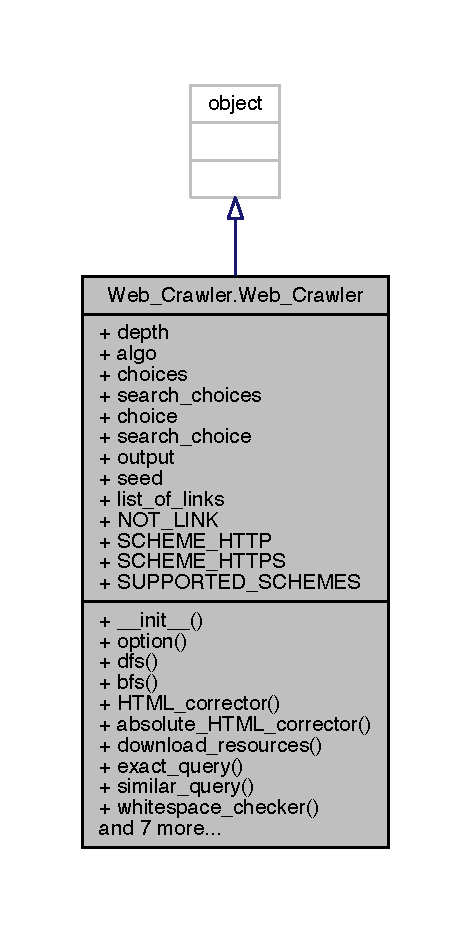
\includegraphics[width=226pt]{class_web___crawler_1_1_web___crawler__inherit__graph}
\end{center}
\end{figure}


Collaboration diagram for Web\+\_\+\+Crawler.\+Web\+\_\+\+Crawler\+:
\nopagebreak
\begin{figure}[H]
\begin{center}
\leavevmode
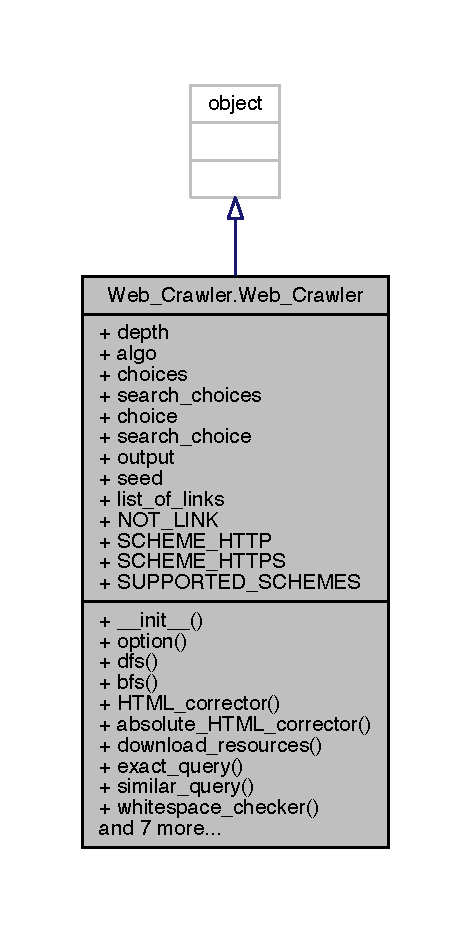
\includegraphics[width=226pt]{class_web___crawler_1_1_web___crawler__coll__graph}
\end{center}
\end{figure}
\subsection*{Public Member Functions}
\begin{DoxyCompactItemize}
\item 
def {\bfseries \+\_\+\+\_\+init\+\_\+\+\_\+} (self)\hypertarget{class_web___crawler_1_1_web___crawler_aa3903156d6d4e8c904c28b14258c239a}{}\label{class_web___crawler_1_1_web___crawler_aa3903156d6d4e8c904c28b14258c239a}

\item 
def \hyperlink{class_web___crawler_1_1_web___crawler_a03625f256ac5f2ce950dd39d8b7e3670}{option} (self)
\item 
def {\bfseries dfs} (self, choice)\hypertarget{class_web___crawler_1_1_web___crawler_a6f9bc2bc5c43de7f05cd068b4af6ba73}{}\label{class_web___crawler_1_1_web___crawler_a6f9bc2bc5c43de7f05cd068b4af6ba73}

\item 
def \hyperlink{class_web___crawler_1_1_web___crawler_a993dac4217f67db152c76c12a2ff9c71}{bfs} (self, link)
\item 
def \hyperlink{class_web___crawler_1_1_web___crawler_a57c901dcd313805cfaf436d005d3c79a}{H\+T\+M\+L\+\_\+corrector} (self, link)
\item 
def \hyperlink{class_web___crawler_1_1_web___crawler_a793dce384c5f064f0fd0974cacb8472c}{absolute\+\_\+\+H\+T\+M\+L\+\_\+corrector} (self, link, base\+\_\+link\+\_\+split)
\item 
def \hyperlink{class_web___crawler_1_1_web___crawler_aacd07e47dfe26cad9229bdc576017c04}{download\+\_\+resources} (self, link, options=\textquotesingle{}-\/rA\textquotesingle{}, file\+\_\+type=None)
\item 
def \hyperlink{class_web___crawler_1_1_web___crawler_afed56534dbc43008f574caad90e0bc68}{exact\+\_\+query} (self, query, data)
\item 
def \hyperlink{class_web___crawler_1_1_web___crawler_a1981e0ead7b4b5b9d3cce3524bb05ebe}{similar\+\_\+query} (self, query, data, proximity)
\item 
def \hyperlink{class_web___crawler_1_1_web___crawler_ac8850d91b2011b6f490d711033e8f191}{whitespace\+\_\+checker} (self, character)
\item 
def \hyperlink{class_web___crawler_1_1_web___crawler_ae2af5c93ae51acf52f8e7efdabab8206}{find\+\_\+links} (self, link, destination=None)
\item 
def \hyperlink{class_web___crawler_1_1_web___crawler_ab027bb04acd098be1ad92d2908f71416}{check\+\_\+errors} (self, link, list\+\_\+of\+\_\+links=None)
\item 
def \hyperlink{class_web___crawler_1_1_web___crawler_abf9ad792a7e19afa406cf793c31f8299}{B\+S\+\_\+parse\+\_\+data} (self, link)
\item 
def \hyperlink{class_web___crawler_1_1_web___crawler_a7353f65405aef84af008bd8fc1eef4f6}{H\+T\+M\+L\+\_\+text} (self, link)
\item 
def \hyperlink{class_web___crawler_1_1_web___crawler_a373e84e41929ee530d250451efbfbc38}{query\+\_\+search} (self, query, link, list\+\_\+of\+\_\+links=None, choice=\textquotesingle{}exact\textquotesingle{})
\item 
def \hyperlink{class_web___crawler_1_1_web___crawler_a7c800e5bc75c0172500fe2d77154a3e7}{depth\+\_\+setter} (self, depth)
\item 
def \hyperlink{class_web___crawler_1_1_web___crawler_a568ddfd327450f38b5b3e8db2355131c}{website\+\_\+structure} (self, link, depth)
\end{DoxyCompactItemize}
\subsection*{Public Attributes}
\begin{DoxyCompactItemize}
\item 
{\bfseries depth}\hypertarget{class_web___crawler_1_1_web___crawler_a46d62130b65d19087c1730728e69e7f1}{}\label{class_web___crawler_1_1_web___crawler_a46d62130b65d19087c1730728e69e7f1}

\item 
{\bfseries algo}\hypertarget{class_web___crawler_1_1_web___crawler_a8ddf9357813b4ac582022543138091c7}{}\label{class_web___crawler_1_1_web___crawler_a8ddf9357813b4ac582022543138091c7}

\item 
{\bfseries choices}\hypertarget{class_web___crawler_1_1_web___crawler_a485e004ec93a8414c352097816f0c1ff}{}\label{class_web___crawler_1_1_web___crawler_a485e004ec93a8414c352097816f0c1ff}

\item 
{\bfseries search\+\_\+choices}\hypertarget{class_web___crawler_1_1_web___crawler_af8079a2cc34f6a281ee767c510f10118}{}\label{class_web___crawler_1_1_web___crawler_af8079a2cc34f6a281ee767c510f10118}

\item 
{\bfseries choice}\hypertarget{class_web___crawler_1_1_web___crawler_a6db21dc7df967c0b186abd7e42e98a3d}{}\label{class_web___crawler_1_1_web___crawler_a6db21dc7df967c0b186abd7e42e98a3d}

\item 
{\bfseries search\+\_\+choice}\hypertarget{class_web___crawler_1_1_web___crawler_abbdeb91eb38beac617e8c9dd7f7d3dfb}{}\label{class_web___crawler_1_1_web___crawler_abbdeb91eb38beac617e8c9dd7f7d3dfb}

\item 
{\bfseries output}\hypertarget{class_web___crawler_1_1_web___crawler_a8a15d32ce74b7f48ef626cf5b6636946}{}\label{class_web___crawler_1_1_web___crawler_a8a15d32ce74b7f48ef626cf5b6636946}

\item 
{\bfseries seed}\hypertarget{class_web___crawler_1_1_web___crawler_a6193cb7d1abb9f19be819009dd212365}{}\label{class_web___crawler_1_1_web___crawler_a6193cb7d1abb9f19be819009dd212365}

\item 
{\bfseries list\+\_\+of\+\_\+links}\hypertarget{class_web___crawler_1_1_web___crawler_a6ebf3939def6aa55af08152a070fc00c}{}\label{class_web___crawler_1_1_web___crawler_a6ebf3939def6aa55af08152a070fc00c}

\item 
{\bfseries N\+O\+T\+\_\+\+L\+I\+NK}\hypertarget{class_web___crawler_1_1_web___crawler_afc29d8ed81f983bb7cfc5d93c38a81b4}{}\label{class_web___crawler_1_1_web___crawler_afc29d8ed81f983bb7cfc5d93c38a81b4}

\item 
{\bfseries S\+C\+H\+E\+M\+E\+\_\+\+H\+T\+TP}\hypertarget{class_web___crawler_1_1_web___crawler_a8f8a86f62cfb6353950e470d75c4f427}{}\label{class_web___crawler_1_1_web___crawler_a8f8a86f62cfb6353950e470d75c4f427}

\item 
{\bfseries S\+C\+H\+E\+M\+E\+\_\+\+H\+T\+T\+PS}\hypertarget{class_web___crawler_1_1_web___crawler_a956b96a3fc5c1e2a770ab2c733196a3c}{}\label{class_web___crawler_1_1_web___crawler_a956b96a3fc5c1e2a770ab2c733196a3c}

\item 
{\bfseries S\+U\+P\+P\+O\+R\+T\+E\+D\+\_\+\+S\+C\+H\+E\+M\+ES}\hypertarget{class_web___crawler_1_1_web___crawler_a8a7e2e14c4659d69cca337d6f18d9531}{}\label{class_web___crawler_1_1_web___crawler_a8a7e2e14c4659d69cca337d6f18d9531}

\end{DoxyCompactItemize}


\subsection{Detailed Description}
\begin{DoxyVerb}Main class, it is for crawling.
Class variable includes depth,algo,choices,choice,output,seed,list of links
\end{DoxyVerb}
 

\subsection{Member Function Documentation}
\index{Web\+\_\+\+Crawler\+::\+Web\+\_\+\+Crawler@{Web\+\_\+\+Crawler\+::\+Web\+\_\+\+Crawler}!absolute\+\_\+\+H\+T\+M\+L\+\_\+corrector@{absolute\+\_\+\+H\+T\+M\+L\+\_\+corrector}}
\index{absolute\+\_\+\+H\+T\+M\+L\+\_\+corrector@{absolute\+\_\+\+H\+T\+M\+L\+\_\+corrector}!Web\+\_\+\+Crawler\+::\+Web\+\_\+\+Crawler@{Web\+\_\+\+Crawler\+::\+Web\+\_\+\+Crawler}}
\subsubsection[{absolute\+\_\+\+H\+T\+M\+L\+\_\+corrector(self, link, base\+\_\+link\+\_\+split)}]{\setlength{\rightskip}{0pt plus 5cm}def Web\+\_\+\+Crawler.\+Web\+\_\+\+Crawler.\+absolute\+\_\+\+H\+T\+M\+L\+\_\+corrector (
\begin{DoxyParamCaption}
\item[{}]{self, }
\item[{}]{link, }
\item[{}]{base\+\_\+link\+\_\+split}
\end{DoxyParamCaption}
)}\hypertarget{class_web___crawler_1_1_web___crawler_a793dce384c5f064f0fd0974cacb8472c}{}\label{class_web___crawler_1_1_web___crawler_a793dce384c5f064f0fd0974cacb8472c}
\begin{DoxyVerb}Takes in the base url and appends any relative or absolute links to the base urk.

:param link:
:param base_link_split:
:return Url object of split url result corrected link Ex; SplitResult(scheme=u'http', netloc=u'canvasgroup.ca', path=u'/zdfzd', query=u'', fragment=u'') ::
\end{DoxyVerb}
 

Here is the call graph for this function\+:
\nopagebreak
\begin{figure}[H]
\begin{center}
\leavevmode
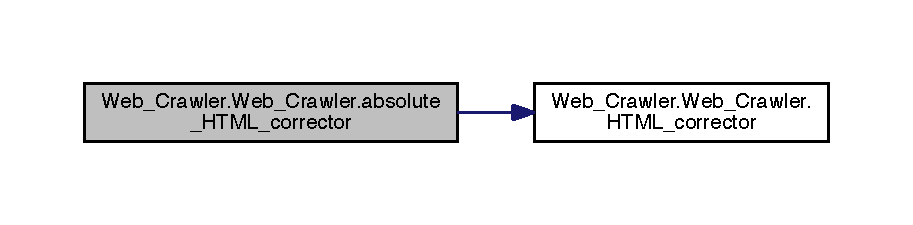
\includegraphics[width=350pt]{class_web___crawler_1_1_web___crawler_a793dce384c5f064f0fd0974cacb8472c_cgraph}
\end{center}
\end{figure}




Here is the caller graph for this function\+:
\nopagebreak
\begin{figure}[H]
\begin{center}
\leavevmode
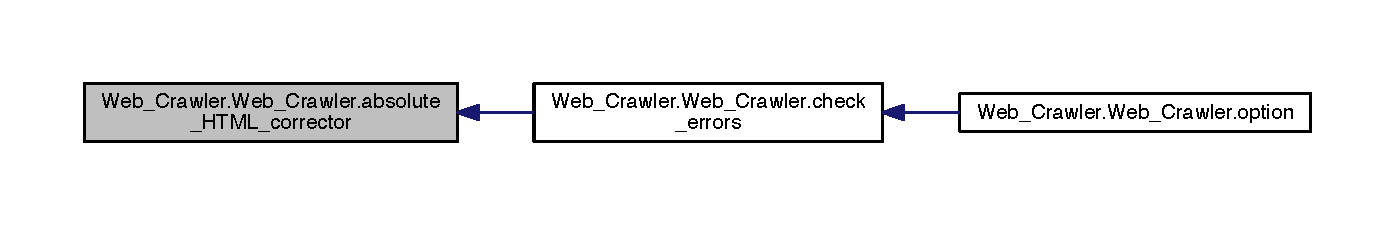
\includegraphics[width=350pt]{class_web___crawler_1_1_web___crawler_a793dce384c5f064f0fd0974cacb8472c_icgraph}
\end{center}
\end{figure}


\index{Web\+\_\+\+Crawler\+::\+Web\+\_\+\+Crawler@{Web\+\_\+\+Crawler\+::\+Web\+\_\+\+Crawler}!bfs@{bfs}}
\index{bfs@{bfs}!Web\+\_\+\+Crawler\+::\+Web\+\_\+\+Crawler@{Web\+\_\+\+Crawler\+::\+Web\+\_\+\+Crawler}}
\subsubsection[{bfs(self, link)}]{\setlength{\rightskip}{0pt plus 5cm}def Web\+\_\+\+Crawler.\+Web\+\_\+\+Crawler.\+bfs (
\begin{DoxyParamCaption}
\item[{}]{self, }
\item[{}]{link}
\end{DoxyParamCaption}
)}\hypertarget{class_web___crawler_1_1_web___crawler_a993dac4217f67db152c76c12a2ff9c71}{}\label{class_web___crawler_1_1_web___crawler_a993dac4217f67db152c76c12a2ff9c71}
\begin{DoxyVerb}Finds all the links on a give website using the BFS algorithm
:param link:
:return A list of all the links found by BFS:
\end{DoxyVerb}
 \index{Web\+\_\+\+Crawler\+::\+Web\+\_\+\+Crawler@{Web\+\_\+\+Crawler\+::\+Web\+\_\+\+Crawler}!B\+S\+\_\+parse\+\_\+data@{B\+S\+\_\+parse\+\_\+data}}
\index{B\+S\+\_\+parse\+\_\+data@{B\+S\+\_\+parse\+\_\+data}!Web\+\_\+\+Crawler\+::\+Web\+\_\+\+Crawler@{Web\+\_\+\+Crawler\+::\+Web\+\_\+\+Crawler}}
\subsubsection[{B\+S\+\_\+parse\+\_\+data(self, link)}]{\setlength{\rightskip}{0pt plus 5cm}def Web\+\_\+\+Crawler.\+Web\+\_\+\+Crawler.\+B\+S\+\_\+parse\+\_\+data (
\begin{DoxyParamCaption}
\item[{}]{self, }
\item[{}]{link}
\end{DoxyParamCaption}
)}\hypertarget{class_web___crawler_1_1_web___crawler_abf9ad792a7e19afa406cf793c31f8299}{}\label{class_web___crawler_1_1_web___crawler_abf9ad792a7e19afa406cf793c31f8299}
\begin{DoxyVerb}Returns BeautifulSoup object for the link given, this will allow modules parse through pages data much faster

:param link:
:return BeautifulSoup :
\end{DoxyVerb}
 

Here is the caller graph for this function\+:
\nopagebreak
\begin{figure}[H]
\begin{center}
\leavevmode
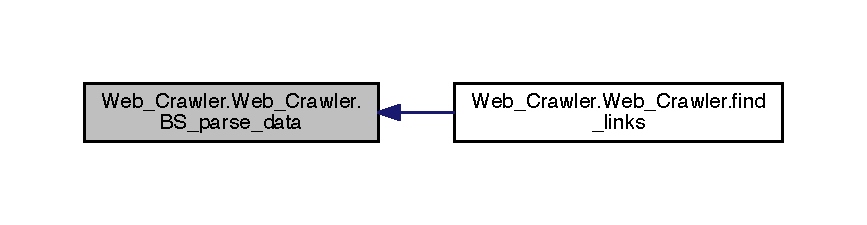
\includegraphics[width=350pt]{class_web___crawler_1_1_web___crawler_abf9ad792a7e19afa406cf793c31f8299_icgraph}
\end{center}
\end{figure}


\index{Web\+\_\+\+Crawler\+::\+Web\+\_\+\+Crawler@{Web\+\_\+\+Crawler\+::\+Web\+\_\+\+Crawler}!check\+\_\+errors@{check\+\_\+errors}}
\index{check\+\_\+errors@{check\+\_\+errors}!Web\+\_\+\+Crawler\+::\+Web\+\_\+\+Crawler@{Web\+\_\+\+Crawler\+::\+Web\+\_\+\+Crawler}}
\subsubsection[{check\+\_\+errors(self, link, list\+\_\+of\+\_\+links=\+None)}]{\setlength{\rightskip}{0pt plus 5cm}def Web\+\_\+\+Crawler.\+Web\+\_\+\+Crawler.\+check\+\_\+errors (
\begin{DoxyParamCaption}
\item[{}]{self, }
\item[{}]{link, }
\item[{}]{list\+\_\+of\+\_\+links = {\ttfamily None}}
\end{DoxyParamCaption}
)}\hypertarget{class_web___crawler_1_1_web___crawler_ab027bb04acd098be1ad92d2908f71416}{}\label{class_web___crawler_1_1_web___crawler_ab027bb04acd098be1ad92d2908f71416}
\begin{DoxyVerb}Checks the all the links and reports the error message associated with
all the links inputted

:param link:
:param list_of_links:
:return List of Errors:
\end{DoxyVerb}
 

Here is the call graph for this function\+:
\nopagebreak
\begin{figure}[H]
\begin{center}
\leavevmode
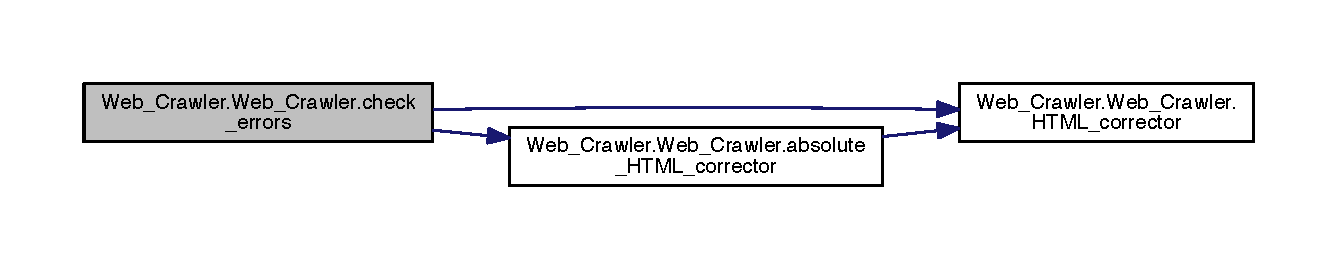
\includegraphics[width=350pt]{class_web___crawler_1_1_web___crawler_ab027bb04acd098be1ad92d2908f71416_cgraph}
\end{center}
\end{figure}




Here is the caller graph for this function\+:
\nopagebreak
\begin{figure}[H]
\begin{center}
\leavevmode
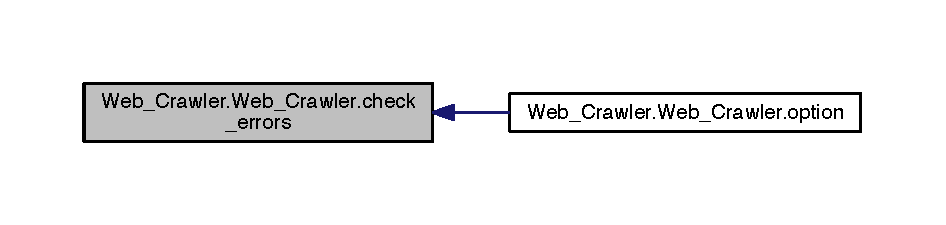
\includegraphics[width=350pt]{class_web___crawler_1_1_web___crawler_ab027bb04acd098be1ad92d2908f71416_icgraph}
\end{center}
\end{figure}


\index{Web\+\_\+\+Crawler\+::\+Web\+\_\+\+Crawler@{Web\+\_\+\+Crawler\+::\+Web\+\_\+\+Crawler}!depth\+\_\+setter@{depth\+\_\+setter}}
\index{depth\+\_\+setter@{depth\+\_\+setter}!Web\+\_\+\+Crawler\+::\+Web\+\_\+\+Crawler@{Web\+\_\+\+Crawler\+::\+Web\+\_\+\+Crawler}}
\subsubsection[{depth\+\_\+setter(self, depth)}]{\setlength{\rightskip}{0pt plus 5cm}def Web\+\_\+\+Crawler.\+Web\+\_\+\+Crawler.\+depth\+\_\+setter (
\begin{DoxyParamCaption}
\item[{}]{self, }
\item[{}]{depth}
\end{DoxyParamCaption}
)}\hypertarget{class_web___crawler_1_1_web___crawler_a7c800e5bc75c0172500fe2d77154a3e7}{}\label{class_web___crawler_1_1_web___crawler_a7c800e5bc75c0172500fe2d77154a3e7}
\begin{DoxyVerb}Sets the default max depth variable for the web crawler
:param depth:
:return:
\end{DoxyVerb}
 

Here is the caller graph for this function\+:
\nopagebreak
\begin{figure}[H]
\begin{center}
\leavevmode
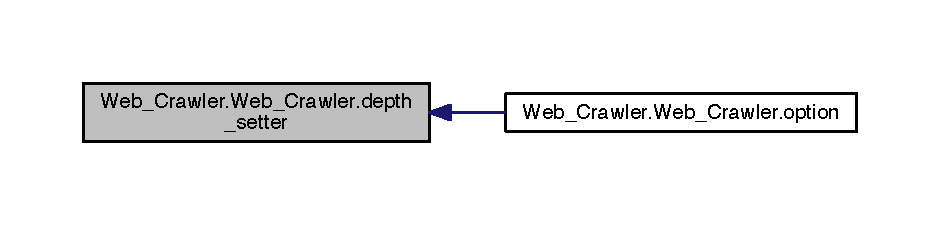
\includegraphics[width=350pt]{class_web___crawler_1_1_web___crawler_a7c800e5bc75c0172500fe2d77154a3e7_icgraph}
\end{center}
\end{figure}


\index{Web\+\_\+\+Crawler\+::\+Web\+\_\+\+Crawler@{Web\+\_\+\+Crawler\+::\+Web\+\_\+\+Crawler}!download\+\_\+resources@{download\+\_\+resources}}
\index{download\+\_\+resources@{download\+\_\+resources}!Web\+\_\+\+Crawler\+::\+Web\+\_\+\+Crawler@{Web\+\_\+\+Crawler\+::\+Web\+\_\+\+Crawler}}
\subsubsection[{download\+\_\+resources(self, link, options=\textquotesingle{}-\/r\+A\textquotesingle{}, file\+\_\+type=\+None)}]{\setlength{\rightskip}{0pt plus 5cm}def Web\+\_\+\+Crawler.\+Web\+\_\+\+Crawler.\+download\+\_\+resources (
\begin{DoxyParamCaption}
\item[{}]{self, }
\item[{}]{link, }
\item[{}]{options = {\ttfamily \textquotesingle{}-\/rA\textquotesingle{}}, }
\item[{}]{file\+\_\+type = {\ttfamily None}}
\end{DoxyParamCaption}
)}\hypertarget{class_web___crawler_1_1_web___crawler_aacd07e47dfe26cad9229bdc576017c04}{}\label{class_web___crawler_1_1_web___crawler_aacd07e47dfe26cad9229bdc576017c04}
\begin{DoxyVerb}Writes all resources matching the given file type from the page link to the file specified by destination.

:param link:
:param options:
:param file_type:
:return:
\end{DoxyVerb}
 

Here is the caller graph for this function\+:
\nopagebreak
\begin{figure}[H]
\begin{center}
\leavevmode
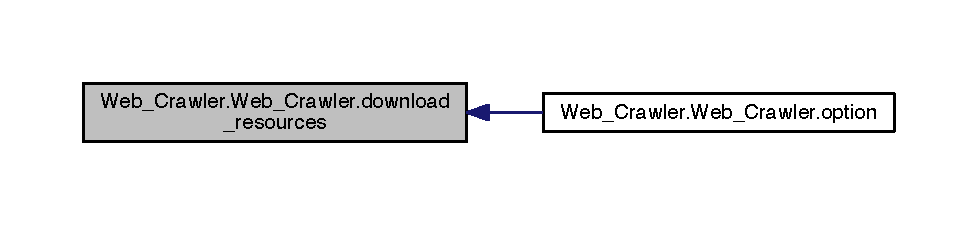
\includegraphics[width=350pt]{class_web___crawler_1_1_web___crawler_aacd07e47dfe26cad9229bdc576017c04_icgraph}
\end{center}
\end{figure}


\index{Web\+\_\+\+Crawler\+::\+Web\+\_\+\+Crawler@{Web\+\_\+\+Crawler\+::\+Web\+\_\+\+Crawler}!exact\+\_\+query@{exact\+\_\+query}}
\index{exact\+\_\+query@{exact\+\_\+query}!Web\+\_\+\+Crawler\+::\+Web\+\_\+\+Crawler@{Web\+\_\+\+Crawler\+::\+Web\+\_\+\+Crawler}}
\subsubsection[{exact\+\_\+query(self, query, data)}]{\setlength{\rightskip}{0pt plus 5cm}def Web\+\_\+\+Crawler.\+Web\+\_\+\+Crawler.\+exact\+\_\+query (
\begin{DoxyParamCaption}
\item[{}]{self, }
\item[{}]{query, }
\item[{}]{data}
\end{DoxyParamCaption}
)}\hypertarget{class_web___crawler_1_1_web___crawler_afed56534dbc43008f574caad90e0bc68}{}\label{class_web___crawler_1_1_web___crawler_afed56534dbc43008f574caad90e0bc68}
\begin{DoxyVerb}Searches through a String for a certain phrase or term. Returns the starting index for all occurrences of the query String.
If the query is not located, it will return an empty array.

:param query - The String we are looking for:
:param data - The String we are searching through.:
:return Indexes corresponding to the beginning of the location of the String in question.:
\end{DoxyVerb}
 

Here is the caller graph for this function\+:
\nopagebreak
\begin{figure}[H]
\begin{center}
\leavevmode
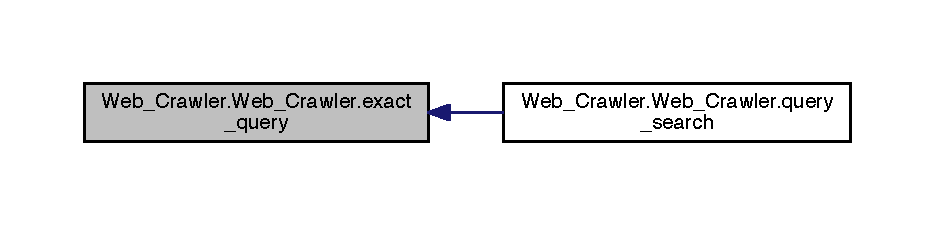
\includegraphics[width=350pt]{class_web___crawler_1_1_web___crawler_afed56534dbc43008f574caad90e0bc68_icgraph}
\end{center}
\end{figure}


\index{Web\+\_\+\+Crawler\+::\+Web\+\_\+\+Crawler@{Web\+\_\+\+Crawler\+::\+Web\+\_\+\+Crawler}!find\+\_\+links@{find\+\_\+links}}
\index{find\+\_\+links@{find\+\_\+links}!Web\+\_\+\+Crawler\+::\+Web\+\_\+\+Crawler@{Web\+\_\+\+Crawler\+::\+Web\+\_\+\+Crawler}}
\subsubsection[{find\+\_\+links(self, link, destination=\+None)}]{\setlength{\rightskip}{0pt plus 5cm}def Web\+\_\+\+Crawler.\+Web\+\_\+\+Crawler.\+find\+\_\+links (
\begin{DoxyParamCaption}
\item[{}]{self, }
\item[{}]{link, }
\item[{}]{destination = {\ttfamily None}}
\end{DoxyParamCaption}
)}\hypertarget{class_web___crawler_1_1_web___crawler_ae2af5c93ae51acf52f8e7efdabab8206}{}\label{class_web___crawler_1_1_web___crawler_ae2af5c93ae51acf52f8e7efdabab8206}
\begin{DoxyVerb}Finds all the links (<a></a> anchor tags on page) on a page, also removes all
the link that start with '#' or 'data:' as these are not valid urls

:param link:
:param destination:
:return List of Links:
\end{DoxyVerb}
 

Here is the call graph for this function\+:
\nopagebreak
\begin{figure}[H]
\begin{center}
\leavevmode
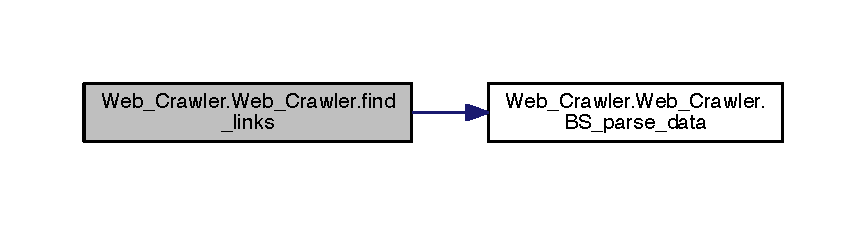
\includegraphics[width=350pt]{class_web___crawler_1_1_web___crawler_ae2af5c93ae51acf52f8e7efdabab8206_cgraph}
\end{center}
\end{figure}


\index{Web\+\_\+\+Crawler\+::\+Web\+\_\+\+Crawler@{Web\+\_\+\+Crawler\+::\+Web\+\_\+\+Crawler}!H\+T\+M\+L\+\_\+corrector@{H\+T\+M\+L\+\_\+corrector}}
\index{H\+T\+M\+L\+\_\+corrector@{H\+T\+M\+L\+\_\+corrector}!Web\+\_\+\+Crawler\+::\+Web\+\_\+\+Crawler@{Web\+\_\+\+Crawler\+::\+Web\+\_\+\+Crawler}}
\subsubsection[{H\+T\+M\+L\+\_\+corrector(self, link)}]{\setlength{\rightskip}{0pt plus 5cm}def Web\+\_\+\+Crawler.\+Web\+\_\+\+Crawler.\+H\+T\+M\+L\+\_\+corrector (
\begin{DoxyParamCaption}
\item[{}]{self, }
\item[{}]{link}
\end{DoxyParamCaption}
)}\hypertarget{class_web___crawler_1_1_web___crawler_a57c901dcd313805cfaf436d005d3c79a}{}\label{class_web___crawler_1_1_web___crawler_a57c901dcd313805cfaf436d005d3c79a}
\begin{DoxyVerb}Fixes the link passed in such that it becomes either a functioning link or is flagged as a broken link.
:param link:
:return  Url object of split url result corrected link Ex; SplitResult(scheme=u'http', netloc=u'canvasgroup.ca', path=u'/zdfzd', query=u'', fragment=u'') :
\end{DoxyVerb}
 

Here is the caller graph for this function\+:
\nopagebreak
\begin{figure}[H]
\begin{center}
\leavevmode
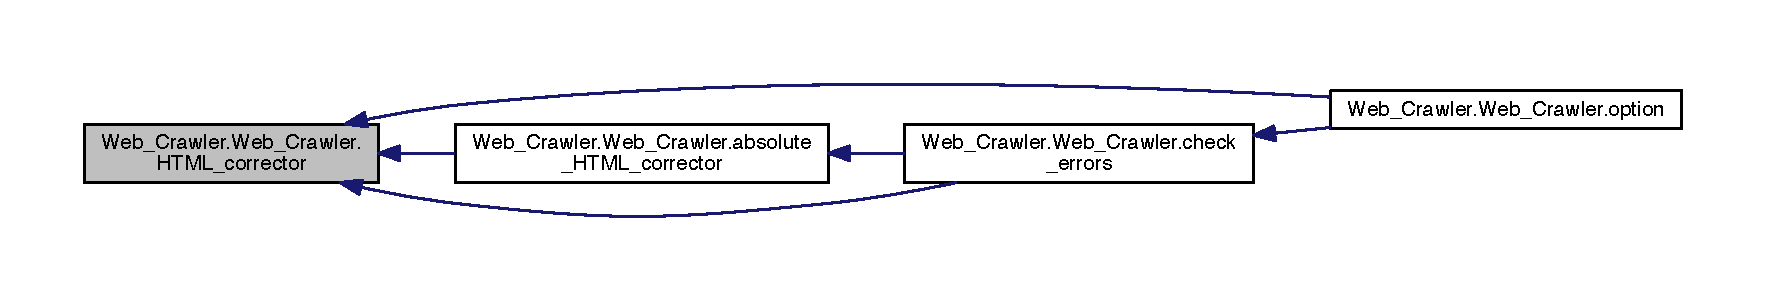
\includegraphics[width=350pt]{class_web___crawler_1_1_web___crawler_a57c901dcd313805cfaf436d005d3c79a_icgraph}
\end{center}
\end{figure}


\index{Web\+\_\+\+Crawler\+::\+Web\+\_\+\+Crawler@{Web\+\_\+\+Crawler\+::\+Web\+\_\+\+Crawler}!H\+T\+M\+L\+\_\+text@{H\+T\+M\+L\+\_\+text}}
\index{H\+T\+M\+L\+\_\+text@{H\+T\+M\+L\+\_\+text}!Web\+\_\+\+Crawler\+::\+Web\+\_\+\+Crawler@{Web\+\_\+\+Crawler\+::\+Web\+\_\+\+Crawler}}
\subsubsection[{H\+T\+M\+L\+\_\+text(self, link)}]{\setlength{\rightskip}{0pt plus 5cm}def Web\+\_\+\+Crawler.\+Web\+\_\+\+Crawler.\+H\+T\+M\+L\+\_\+text (
\begin{DoxyParamCaption}
\item[{}]{self, }
\item[{}]{link}
\end{DoxyParamCaption}
)}\hypertarget{class_web___crawler_1_1_web___crawler_a7353f65405aef84af008bd8fc1eef4f6}{}\label{class_web___crawler_1_1_web___crawler_a7353f65405aef84af008bd8fc1eef4f6}
\begin{DoxyVerb}Returns HTML text data for Query search

:param link:
:return String :
\end{DoxyVerb}
 

Here is the caller graph for this function\+:
\nopagebreak
\begin{figure}[H]
\begin{center}
\leavevmode
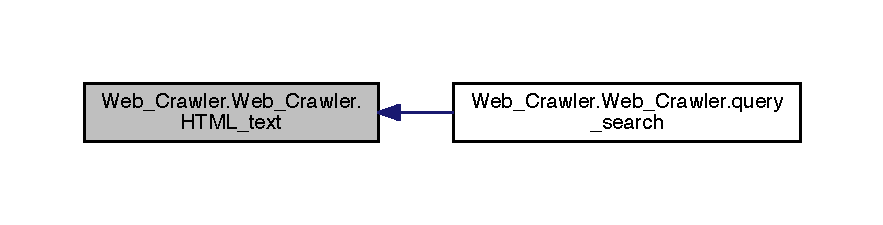
\includegraphics[width=350pt]{class_web___crawler_1_1_web___crawler_a7353f65405aef84af008bd8fc1eef4f6_icgraph}
\end{center}
\end{figure}


\index{Web\+\_\+\+Crawler\+::\+Web\+\_\+\+Crawler@{Web\+\_\+\+Crawler\+::\+Web\+\_\+\+Crawler}!option@{option}}
\index{option@{option}!Web\+\_\+\+Crawler\+::\+Web\+\_\+\+Crawler@{Web\+\_\+\+Crawler\+::\+Web\+\_\+\+Crawler}}
\subsubsection[{option(self)}]{\setlength{\rightskip}{0pt plus 5cm}def Web\+\_\+\+Crawler.\+Web\+\_\+\+Crawler.\+option (
\begin{DoxyParamCaption}
\item[{}]{self}
\end{DoxyParamCaption}
)}\hypertarget{class_web___crawler_1_1_web___crawler_a03625f256ac5f2ce950dd39d8b7e3670}{}\label{class_web___crawler_1_1_web___crawler_a03625f256ac5f2ce950dd39d8b7e3670}
\begin{DoxyVerb}Gets user input to set various program options related to
how the user would like to handle crawling a webpage.

Ask for users option choices

:return:
\end{DoxyVerb}
 

Here is the call graph for this function\+:
\nopagebreak
\begin{figure}[H]
\begin{center}
\leavevmode
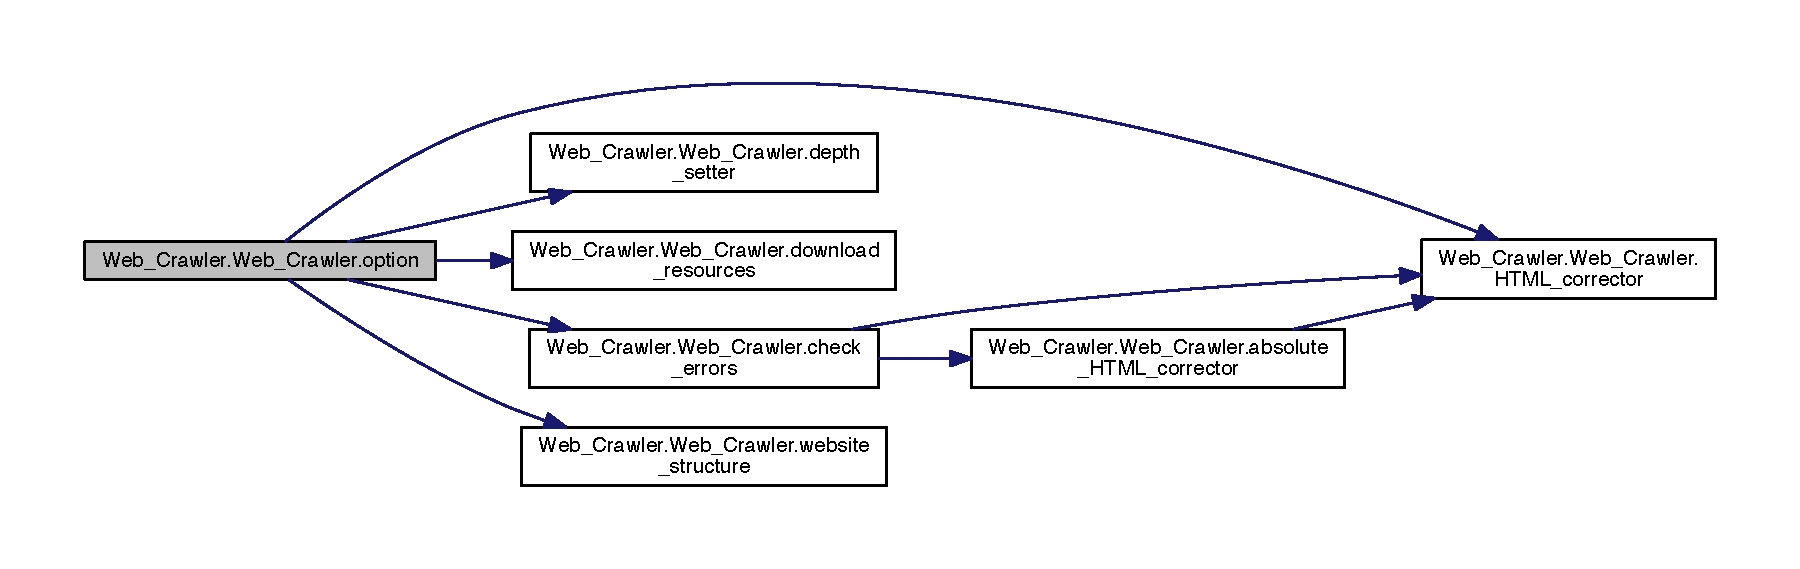
\includegraphics[width=350pt]{class_web___crawler_1_1_web___crawler_a03625f256ac5f2ce950dd39d8b7e3670_cgraph}
\end{center}
\end{figure}


\index{Web\+\_\+\+Crawler\+::\+Web\+\_\+\+Crawler@{Web\+\_\+\+Crawler\+::\+Web\+\_\+\+Crawler}!query\+\_\+search@{query\+\_\+search}}
\index{query\+\_\+search@{query\+\_\+search}!Web\+\_\+\+Crawler\+::\+Web\+\_\+\+Crawler@{Web\+\_\+\+Crawler\+::\+Web\+\_\+\+Crawler}}
\subsubsection[{query\+\_\+search(self, query, link, list\+\_\+of\+\_\+links=\+None, choice=\textquotesingle{}exact\textquotesingle{})}]{\setlength{\rightskip}{0pt plus 5cm}def Web\+\_\+\+Crawler.\+Web\+\_\+\+Crawler.\+query\+\_\+search (
\begin{DoxyParamCaption}
\item[{}]{self, }
\item[{}]{query, }
\item[{}]{link, }
\item[{}]{list\+\_\+of\+\_\+links = {\ttfamily None}, }
\item[{}]{choice = {\ttfamily \textquotesingle{}exact\textquotesingle{}}}
\end{DoxyParamCaption}
)}\hypertarget{class_web___crawler_1_1_web___crawler_a373e84e41929ee530d250451efbfbc38}{}\label{class_web___crawler_1_1_web___crawler_a373e84e41929ee530d250451efbfbc38}
\begin{DoxyVerb}Find queries

:param query:
:param data:
:param choice:
:return Query results:
\end{DoxyVerb}
 

Here is the call graph for this function\+:
\nopagebreak
\begin{figure}[H]
\begin{center}
\leavevmode
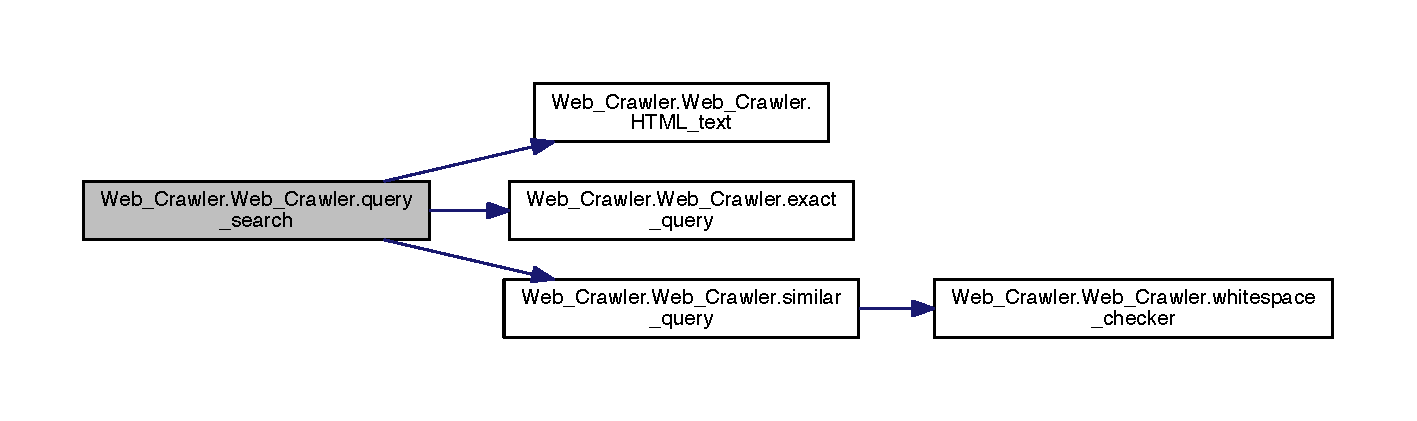
\includegraphics[width=350pt]{class_web___crawler_1_1_web___crawler_a373e84e41929ee530d250451efbfbc38_cgraph}
\end{center}
\end{figure}


\index{Web\+\_\+\+Crawler\+::\+Web\+\_\+\+Crawler@{Web\+\_\+\+Crawler\+::\+Web\+\_\+\+Crawler}!similar\+\_\+query@{similar\+\_\+query}}
\index{similar\+\_\+query@{similar\+\_\+query}!Web\+\_\+\+Crawler\+::\+Web\+\_\+\+Crawler@{Web\+\_\+\+Crawler\+::\+Web\+\_\+\+Crawler}}
\subsubsection[{similar\+\_\+query(self, query, data, proximity)}]{\setlength{\rightskip}{0pt plus 5cm}def Web\+\_\+\+Crawler.\+Web\+\_\+\+Crawler.\+similar\+\_\+query (
\begin{DoxyParamCaption}
\item[{}]{self, }
\item[{}]{query, }
\item[{}]{data, }
\item[{}]{proximity}
\end{DoxyParamCaption}
)}\hypertarget{class_web___crawler_1_1_web___crawler_a1981e0ead7b4b5b9d3cce3524bb05ebe}{}\label{class_web___crawler_1_1_web___crawler_a1981e0ead7b4b5b9d3cce3524bb05ebe}
\begin{DoxyVerb}Searches through a String for a certain phrase or term. Returns results that are close to the query as well.
(i.e. "ap ple" or "bpple" would be noted for "apple") Returns the starting index for all occurrences of Strings sufficiently close to
the query. If the query is not located, it will return an empty array.

:param: query  - The String we are looking for.
:param: data - The String we are searching through.:
:param: proximity - The size of the acceptable variation from the query.:
:return:Indexes corresponding to the beginning of the location of the String in question.
\end{DoxyVerb}
 

Here is the call graph for this function\+:
\nopagebreak
\begin{figure}[H]
\begin{center}
\leavevmode
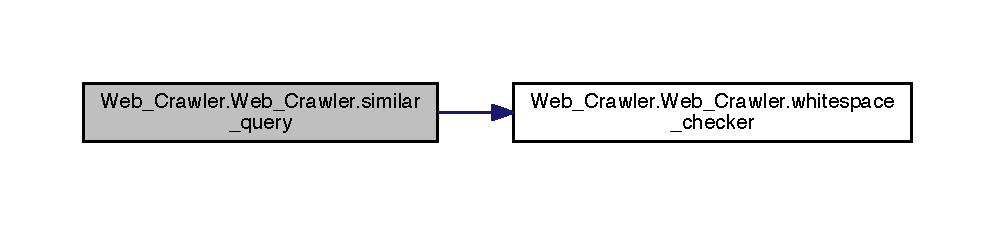
\includegraphics[width=350pt]{class_web___crawler_1_1_web___crawler_a1981e0ead7b4b5b9d3cce3524bb05ebe_cgraph}
\end{center}
\end{figure}




Here is the caller graph for this function\+:
\nopagebreak
\begin{figure}[H]
\begin{center}
\leavevmode
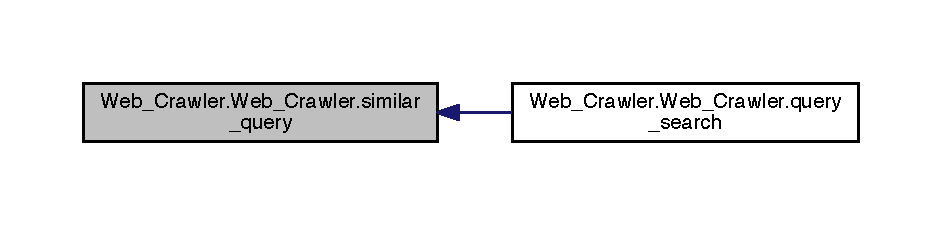
\includegraphics[width=350pt]{class_web___crawler_1_1_web___crawler_a1981e0ead7b4b5b9d3cce3524bb05ebe_icgraph}
\end{center}
\end{figure}


\index{Web\+\_\+\+Crawler\+::\+Web\+\_\+\+Crawler@{Web\+\_\+\+Crawler\+::\+Web\+\_\+\+Crawler}!website\+\_\+structure@{website\+\_\+structure}}
\index{website\+\_\+structure@{website\+\_\+structure}!Web\+\_\+\+Crawler\+::\+Web\+\_\+\+Crawler@{Web\+\_\+\+Crawler\+::\+Web\+\_\+\+Crawler}}
\subsubsection[{website\+\_\+structure(self, link, depth)}]{\setlength{\rightskip}{0pt plus 5cm}def Web\+\_\+\+Crawler.\+Web\+\_\+\+Crawler.\+website\+\_\+structure (
\begin{DoxyParamCaption}
\item[{}]{self, }
\item[{}]{link, }
\item[{}]{depth}
\end{DoxyParamCaption}
)}\hypertarget{class_web___crawler_1_1_web___crawler_a568ddfd327450f38b5b3e8db2355131c}{}\label{class_web___crawler_1_1_web___crawler_a568ddfd327450f38b5b3e8db2355131c}
\begin{DoxyVerb}It provides a structured model of the website and other site the initial site is connect to. It displays
a hierarchy that will show users how crawled link interact with each other. Shows all the depths

:param link:
:param depth:
:return A pretty print of Hierarchy:
\end{DoxyVerb}
 

Here is the caller graph for this function\+:
\nopagebreak
\begin{figure}[H]
\begin{center}
\leavevmode
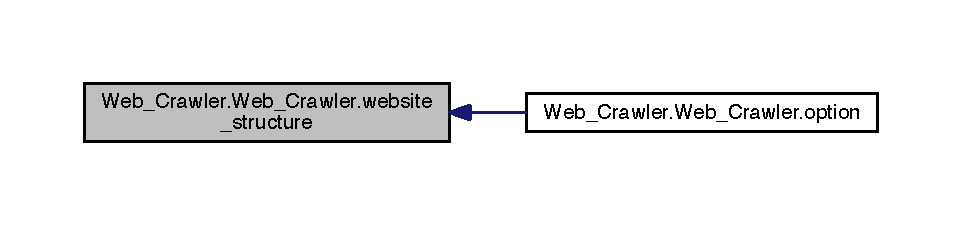
\includegraphics[width=350pt]{class_web___crawler_1_1_web___crawler_a568ddfd327450f38b5b3e8db2355131c_icgraph}
\end{center}
\end{figure}


\index{Web\+\_\+\+Crawler\+::\+Web\+\_\+\+Crawler@{Web\+\_\+\+Crawler\+::\+Web\+\_\+\+Crawler}!whitespace\+\_\+checker@{whitespace\+\_\+checker}}
\index{whitespace\+\_\+checker@{whitespace\+\_\+checker}!Web\+\_\+\+Crawler\+::\+Web\+\_\+\+Crawler@{Web\+\_\+\+Crawler\+::\+Web\+\_\+\+Crawler}}
\subsubsection[{whitespace\+\_\+checker(self, character)}]{\setlength{\rightskip}{0pt plus 5cm}def Web\+\_\+\+Crawler.\+Web\+\_\+\+Crawler.\+whitespace\+\_\+checker (
\begin{DoxyParamCaption}
\item[{}]{self, }
\item[{}]{character}
\end{DoxyParamCaption}
)}\hypertarget{class_web___crawler_1_1_web___crawler_ac8850d91b2011b6f490d711033e8f191}{}\label{class_web___crawler_1_1_web___crawler_ac8850d91b2011b6f490d711033e8f191}
\begin{DoxyVerb}Returns true if the character passed in is a whitespace character such as tab, space or newline.

:param character - The character to be checked.:
:return boolean, if there is whitespace True,Whether the character is whitespace:
\end{DoxyVerb}
 

Here is the caller graph for this function\+:
\nopagebreak
\begin{figure}[H]
\begin{center}
\leavevmode
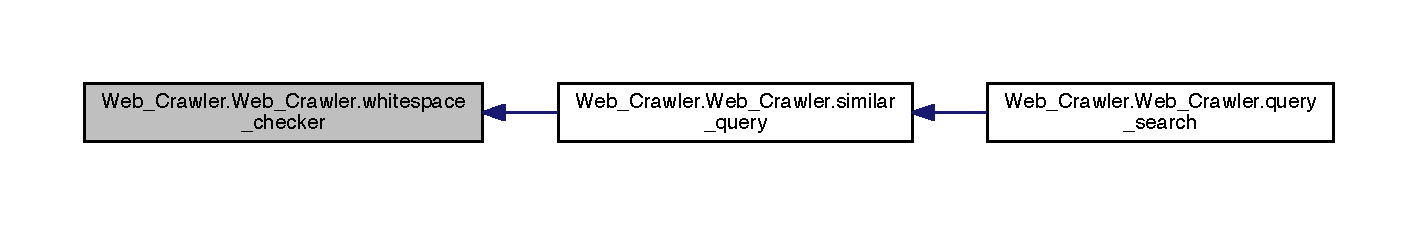
\includegraphics[width=350pt]{class_web___crawler_1_1_web___crawler_ac8850d91b2011b6f490d711033e8f191_icgraph}
\end{center}
\end{figure}




The documentation for this class was generated from the following file\+:\begin{DoxyCompactItemize}
\item 
P\+O\+C Code/Web\+\_\+\+Crawler.\+py\end{DoxyCompactItemize}

\hypertarget{class_web___crawler___p_o_c_1_1_web___crawler___p_o_c}{}\section{Web\+\_\+\+Crawler\+\_\+\+P\+O\+C.\+Web\+\_\+\+Crawler\+\_\+\+P\+OC Class Reference}
\label{class_web___crawler___p_o_c_1_1_web___crawler___p_o_c}\index{Web\+\_\+\+Crawler\+\_\+\+P\+O\+C.\+Web\+\_\+\+Crawler\+\_\+\+P\+OC@{Web\+\_\+\+Crawler\+\_\+\+P\+O\+C.\+Web\+\_\+\+Crawler\+\_\+\+P\+OC}}


Inheritance diagram for Web\+\_\+\+Crawler\+\_\+\+P\+O\+C.\+Web\+\_\+\+Crawler\+\_\+\+P\+OC\+:
\nopagebreak
\begin{figure}[H]
\begin{center}
\leavevmode
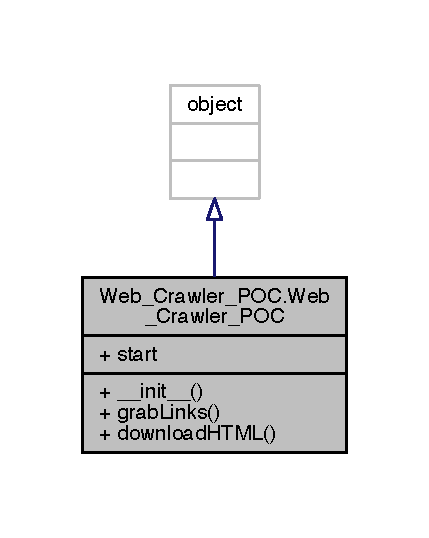
\includegraphics[width=206pt]{class_web___crawler___p_o_c_1_1_web___crawler___p_o_c__inherit__graph}
\end{center}
\end{figure}


Collaboration diagram for Web\+\_\+\+Crawler\+\_\+\+P\+O\+C.\+Web\+\_\+\+Crawler\+\_\+\+P\+OC\+:
\nopagebreak
\begin{figure}[H]
\begin{center}
\leavevmode
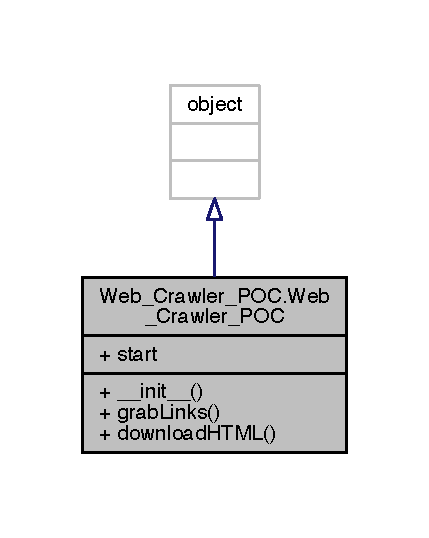
\includegraphics[width=206pt]{class_web___crawler___p_o_c_1_1_web___crawler___p_o_c__coll__graph}
\end{center}
\end{figure}
\subsection*{Public Member Functions}
\begin{DoxyCompactItemize}
\item 
def {\bfseries \+\_\+\+\_\+init\+\_\+\+\_\+} (self)\hypertarget{class_web___crawler___p_o_c_1_1_web___crawler___p_o_c_a232eab61453fcf69417a28bae300d455}{}\label{class_web___crawler___p_o_c_1_1_web___crawler___p_o_c_a232eab61453fcf69417a28bae300d455}

\item 
def {\bfseries grab\+Links} (self)\hypertarget{class_web___crawler___p_o_c_1_1_web___crawler___p_o_c_afefd3071c3d330773bc1cadca2b58801}{}\label{class_web___crawler___p_o_c_1_1_web___crawler___p_o_c_afefd3071c3d330773bc1cadca2b58801}

\item 
def {\bfseries download\+H\+T\+ML} (self)\hypertarget{class_web___crawler___p_o_c_1_1_web___crawler___p_o_c_aa68f01d7c03def373ae2389757c1de89}{}\label{class_web___crawler___p_o_c_1_1_web___crawler___p_o_c_aa68f01d7c03def373ae2389757c1de89}

\end{DoxyCompactItemize}
\subsection*{Public Attributes}
\begin{DoxyCompactItemize}
\item 
{\bfseries start}\hypertarget{class_web___crawler___p_o_c_1_1_web___crawler___p_o_c_a5a87a2533b8d08083270432c3ff658a9}{}\label{class_web___crawler___p_o_c_1_1_web___crawler___p_o_c_a5a87a2533b8d08083270432c3ff658a9}

\end{DoxyCompactItemize}


The documentation for this class was generated from the following file\+:\begin{DoxyCompactItemize}
\item 
P\+O\+C Code/Web\+\_\+\+Crawler\+\_\+\+P\+O\+C.\+py\end{DoxyCompactItemize}

%--- End generated contents ---

% Index
\backmatter
\newpage
\phantomsection
\clearemptydoublepage
\addcontentsline{toc}{chapter}{Index}
\printindex

\end{document}
